\section{Horizontal Shifting}

Now that we are working in grayscale, it is far more straightforward to
manipulate aspects of the image, such as its         horizontal position.
Since we are dealing with a normal matrix, transforming the positions of
columns requires only that    we multiply the image matrix by a
transformation identity matrix.

As discussed in the lab instructions, to shift an image horizontally
without
losing information requires the use of a transformation matrix as shown
below.

\[
  \underbrace{
    \begin{bmatrix}
      1&0&0\\
      0&1&0\\
      0&0&1\\
    \end{bmatrix}
  }_{\text{Identity Matrix}}
  \implies
  \underbrace{
    \begin{bmatrix}
      0&1&0\\
      0&0&1\\
      1&0&0\\
    \end{bmatrix}
  }_{\text{Transformation
  Matrix}}
\]

\[ 
  \begin{bmatrix}
    0&0&1\\
    1&0&0\\
    0&1&0\\
  \end{bmatrix}
  \cdot
  \begin{bmatrix}
    a&b&c\\
    d&e&f\\
    g&h&i\\
  \end{bmatrix}
  =
  \underbrace{
    \begin{bmatrix}
      c&a&b\\
      f&d&e\\
      i&g&h\\
    \end{bmatrix}
  }_{\text{the
    horizontally
    shifted
  matrix}}
\]

\begin{figure}[ht]
  \centering
  \begin{subfigure}{\textwidth}
    \centering
    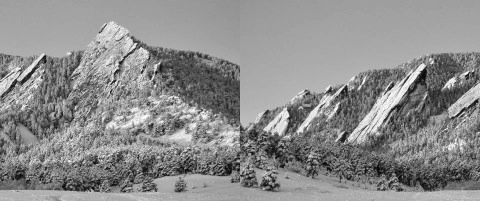
\includegraphics[scale=0.7]{./img/hsg1.png}
    \caption{Photo
      1
      Horizontal
    Shift}
    \label{fig:p1hg}
  \end{subfigure}
  \begin{subfigure}{\textwidth}
    \centering
    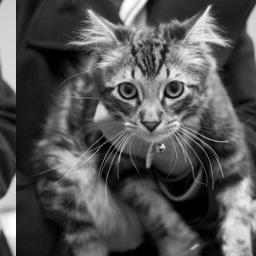
\includegraphics[scale=0.7]{./img/hsg2.png}
    \caption{Photo
      2
      -
      Horizontal
    Shift}
    \label{fig:p2hg}
  \end{subfigure}
  \caption{Horizontally
    Shifted
  Images}
  \label{fig:hs_images}
\end{figure}

